\chapter{Architettura proposta}
	\label{chap:architettura-proposta}
		In questo capitolo sarà descritta l'architettura del framework sviluppato per la conversione di voci a spettro ridotto mediante l'utilizzo di vocoded speech e di sine-wave speech.
		
		\section{Metodo}
		L'idea alla base di questo framework è la conversione di voci tra due speaker differenti che andremo a chiamare $X$ (sorgente) e $Y$ (target).
		
		L'innovazione principale del framework proposto è la riduzione dello spettro sonoro, processo attraverso il quale si riducono le caratteristiche acustiche dello speaker sorgente $X$.
		
		Andremo a presentare due moduli per questo scopo: un modulo di riduzione a sine-wave speech (SWS) e uno di riduzione a vocoded speech.
	
		\begin{figure}[h]
			\centering
			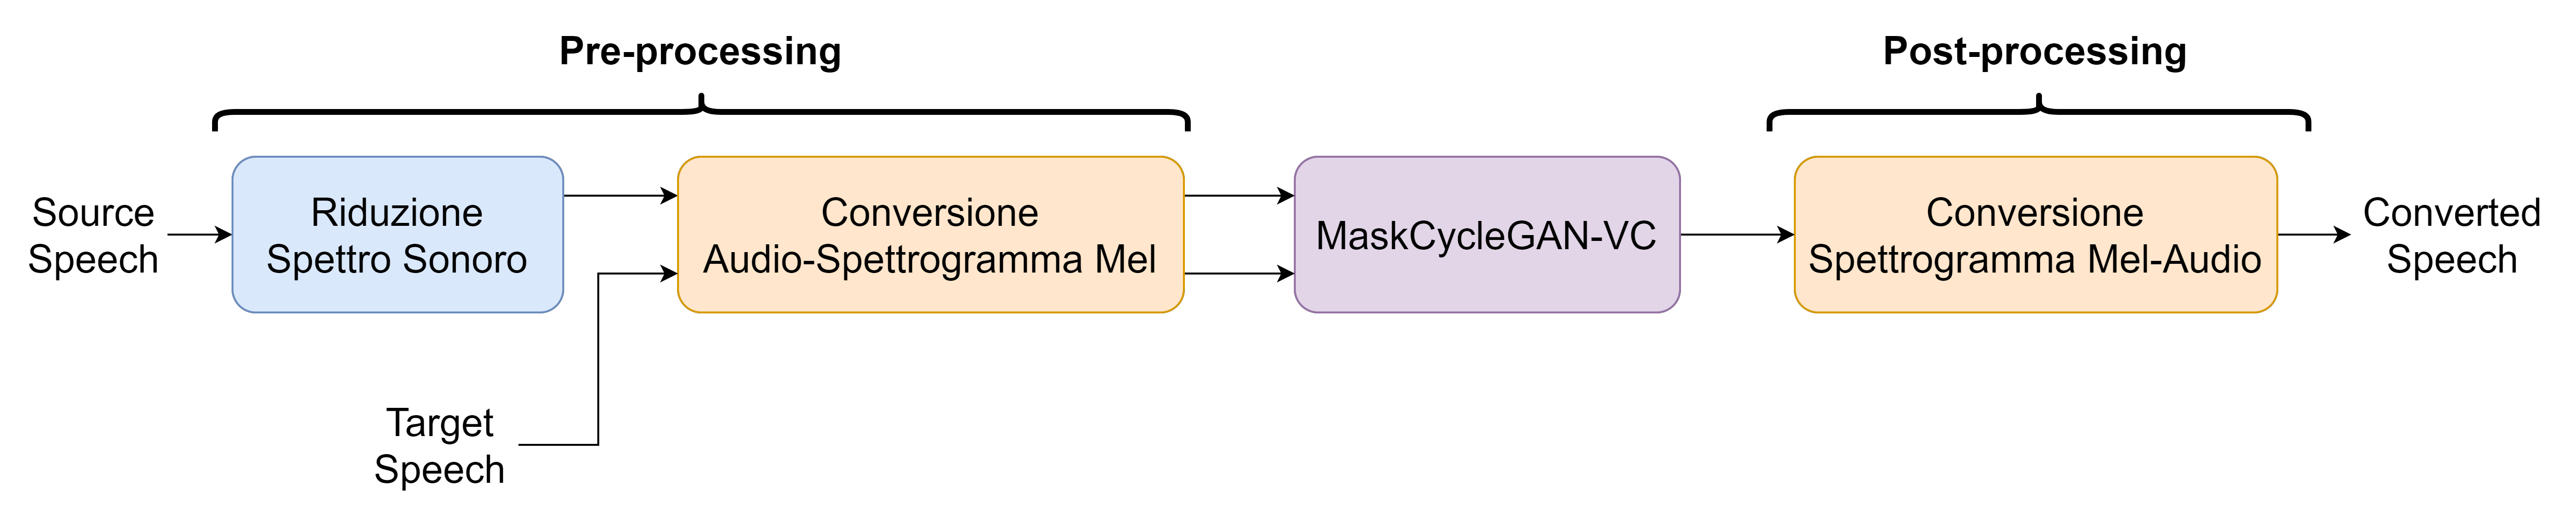
\includegraphics[width=1\linewidth]{figures/MaskCycleGAN-SWS-VC-pipeline}
			\caption{Pipeline dell'architettura proposta.}
			\label{fig:maskcyclegan-sws-vc-pipeline}
		\end{figure}		
		
		\section{Modulo di riduzione dello spettro sonoro}
		\label{sec:proposta-riduzione}
			I seguenti moduli sono parte della fase di pre-processamento dell'audio (Fig. \ref{fig:maskcyclegan-sws-vc-pipeline} e \ref{fig:modulo-riduzione-spettro-sonoro}).			
		
			\subsection{Modulo di riduzione a vocoded speech}
			Il metodo implementato per generare il vocoded speech si basa su Linear Predictive Coding (LPC), impiegando l'algoritmo di Burg\cite{burg-algorithm}.
			Si descrive di seguito la procedura applicata:
			\begin{itemize}
				\item L'audio originale viene ricampionato a 8 kHz. In questo modo la frequenza di Nyquist, che per definizione si attesta a $ \frac{1}{2} f_{s} $, sarà di 4 kHz ovvero sarà possibile rappresentare senza distorsioni suoni fino a tale frequenza. Tale range di frequenze viene usato come banda standard per la voce in comunicazioni telefoniche. 
				\item Vengono estratte finestre di 200 sample dell'audio.
				\item Per ogni finestra vengono calcolati i coefficienti del filtro lineare di ordine 8.
				\item Viene generato un segnale carrier della durata di 200 sample (es. buzz a 500 Hz oppure noise).
				\item Viene applicato un filtro lineare del resiudo LPC al carrier in modo da ricostruire il segnale vocale su di esso.
				\item Viene calcolata la magnitudine della finestra e viene adattato il segnale generato ad essa.
				\item L'audio viene ricostruito e ricampionato alla frequenza originale.
			\end{itemize}
		
			\subsection{Modulo di riduzione a SWS}
			Al fine di trasformare degli audio in forma sine-wave speech abbiamo la necessità di trovare le formanti e rimpiazzarle con delle onde sinusoidali pure. Il metodo implementato si basa sulla stima delle posizioni delle formanti data dalla Linear Predictive Coding (LPC)\cite{formants-from-lpc}, utilizzando l'algoritmo di Burg\cite{burg-algorithm}.
			Si descrive di seguito la procedura applicata:
			\begin{itemize}
				\item L'audio originale viene ricampionato a 8 kHz.
				\item Vengono estratte finestre di 200 sample dell'audio.
				\item Per ogni finestra vengono calcolati i coefficienti del filtro lineare di ordine 12 e si ottengono le frequenze delle formanti. La scelta dell'ordine deriva dalla seguente formula $ o = 2 \cdot n_{f} + 2 $, dove $ n_{f} $ rappresenta il numero delle formanti da trovare.
				\item Viene calcolata la magnitudine della finestra.
				\item Vengono interpolate le formanti al fine di creare 3 segnali sinusoidali mobili.
				\item Si ricostruisce l'audio alla frequenza di campionamento originale con sinusoidi alle frequenze delle formanti.
			\end{itemize}
			\begin{figure}
				\centering
				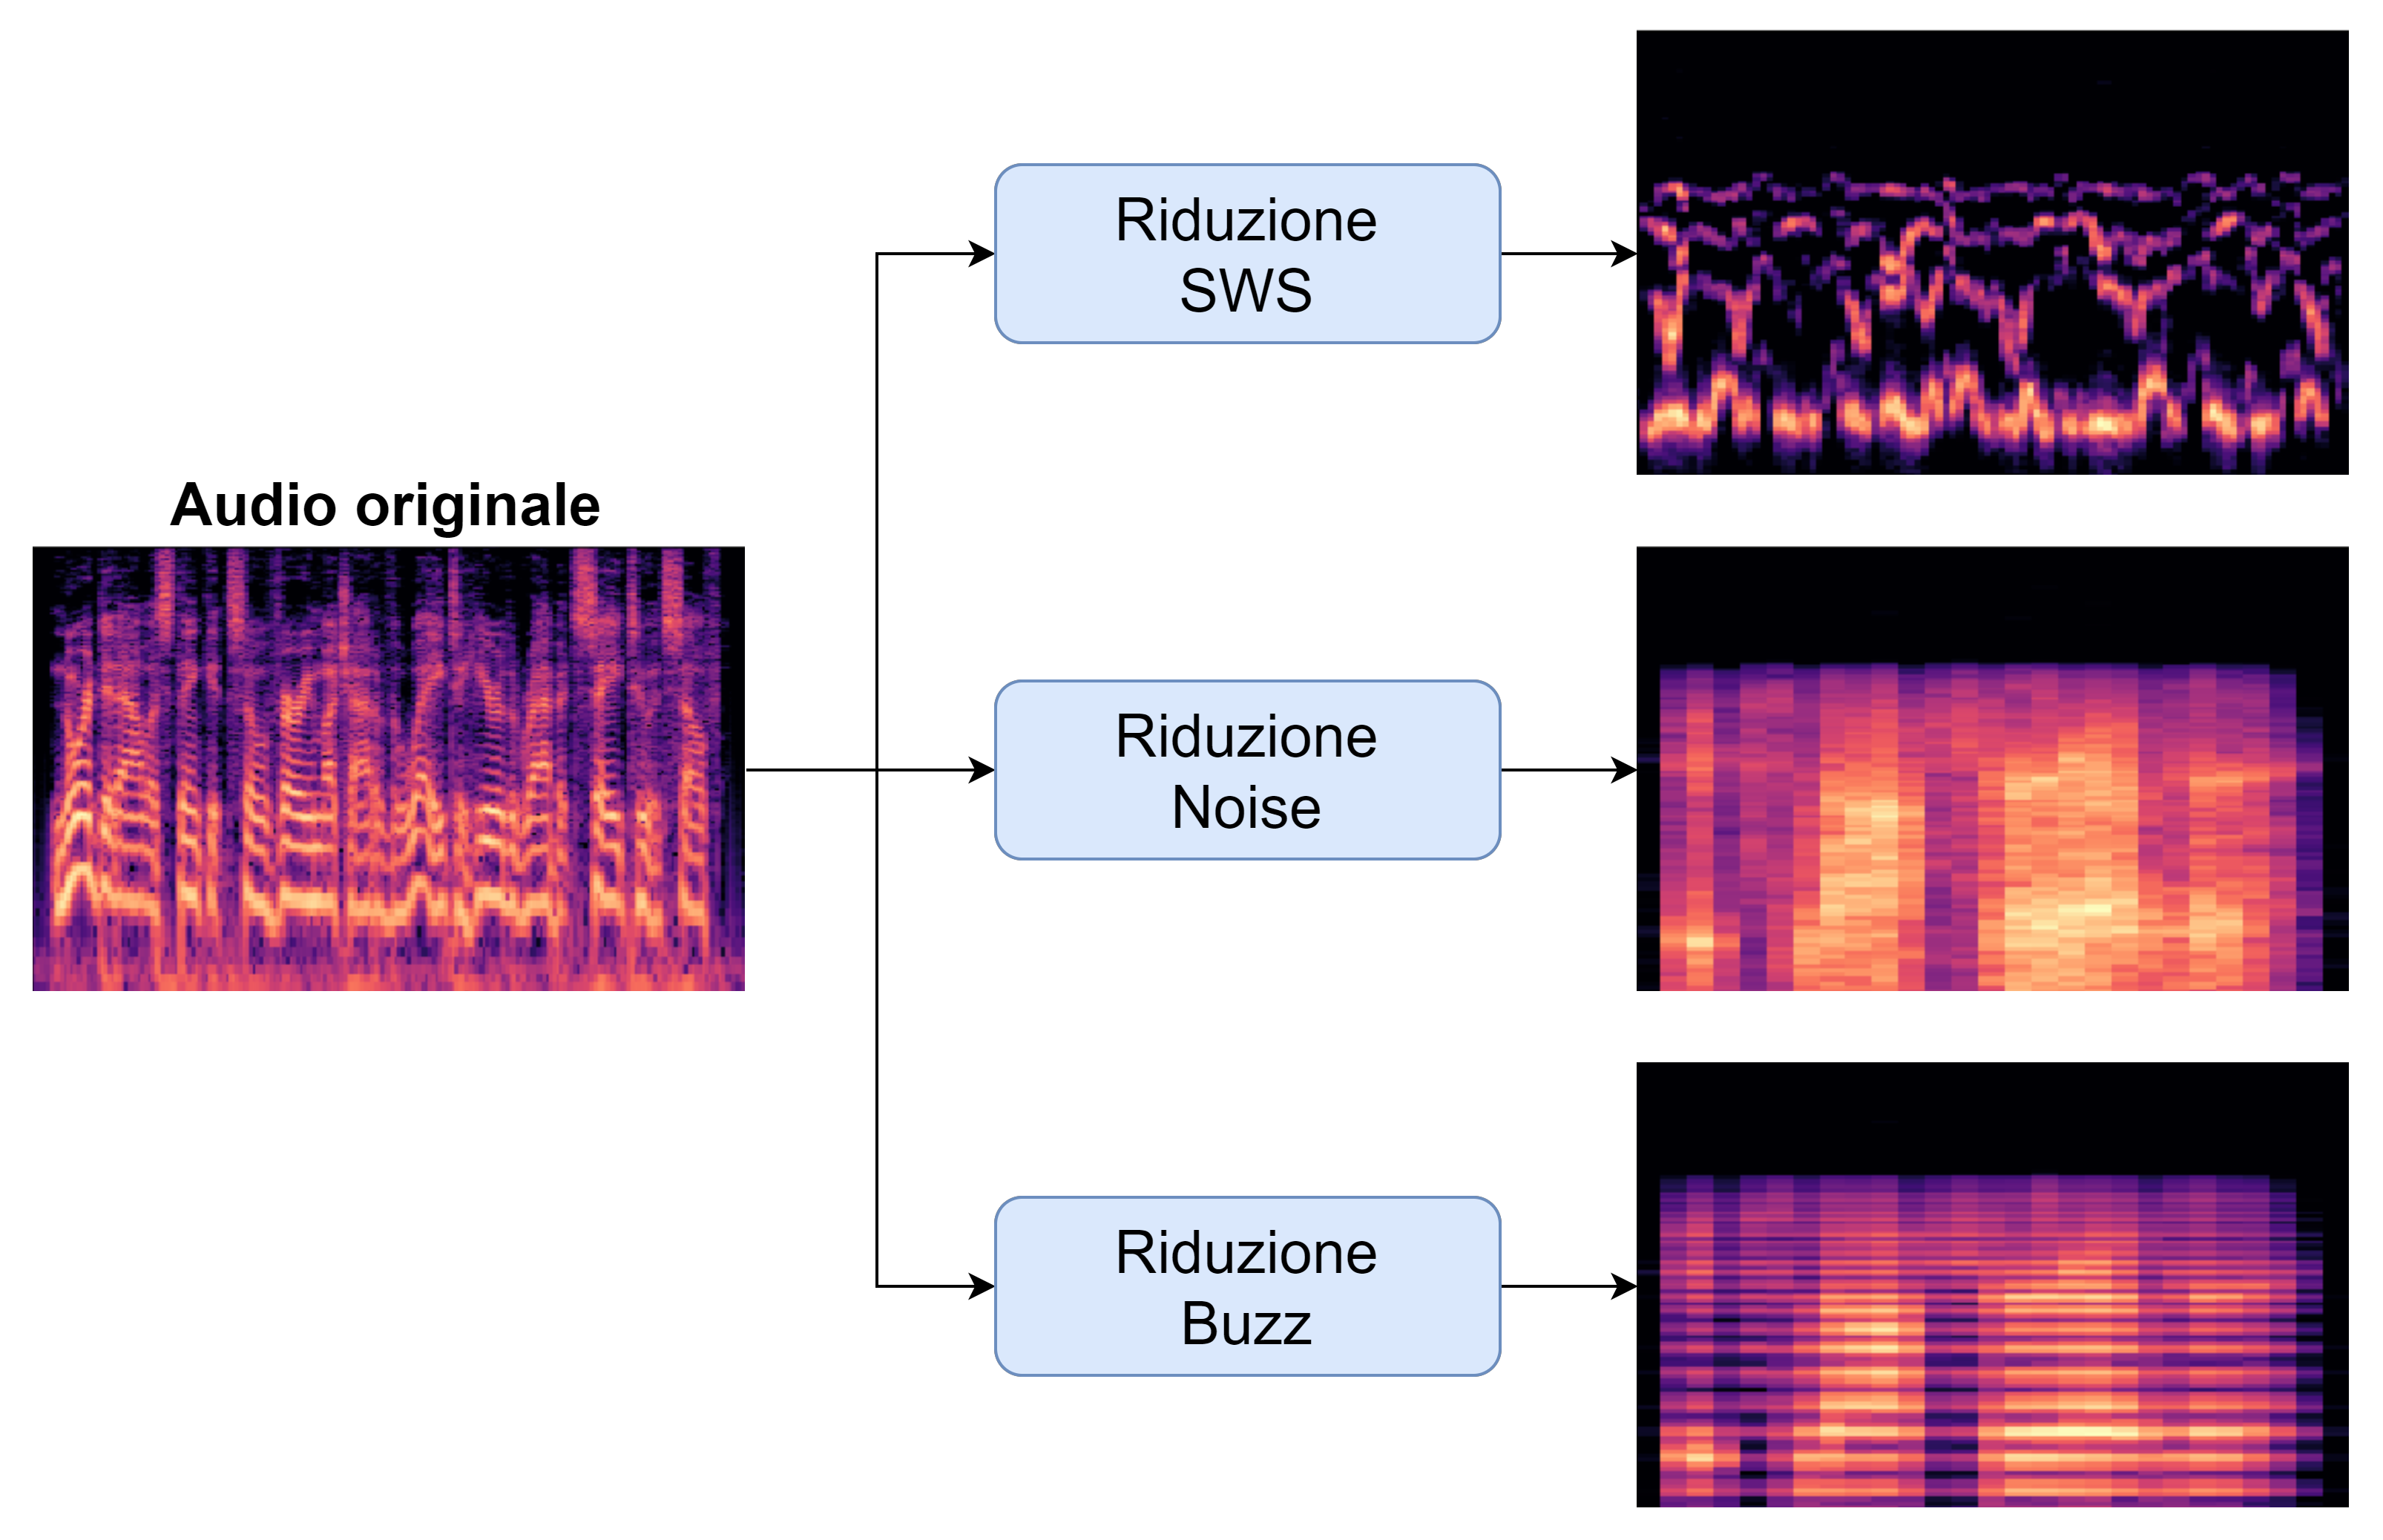
\includegraphics[width=0.8\linewidth]{figures/modulo-riduzione-spettro-sonoro}
				\caption{Risultati della riduzione dello spettro sonoro applicando i tre metodi proposti: sine-wave speech, noise vocoded speech e buzz vocoded speech.}
				\label{fig:modulo-riduzione-spettro-sonoro}
			\end{figure}
	
		\section{Modulo di conversione audio-spettrogrammi}
		Al fine di poter utilizzare la rete MaskCycleGAN-VC è necessario trasformare degli audio in spettrogrammi da fornire come input ad essa e successivamente di invertire questa trasformazione per ottenere un audio in output. È stata scelto di impiegare lo stesso modello utilizzato nel paper di riferimento di Kaneko et al.\cite{MaskCyclegan-VC}, ovvero una MelGAN\cite{melgan} pretrainata, al fine di poter effettuare un confronto più diretto sui risultati ottenuti dalle rappresentazioni scelte come input.
	
		\section{Architettura della rete}
		L'architettura della rete neurale artificiale utilizzata è la MaskCycleGAN-VC come descritta nel \autoref{chap:deep-learning} (Fig. \ref{fig:maskcyclegan-sws-vc}).		
		La scelta di non modificare parametri della rete è voluta al fine di poter ottenere dei risultati oggettivi dipendenti esclusivamente dalla riduzione spettrale proposta.
		
		\begin{figure}[h]
			\centering
			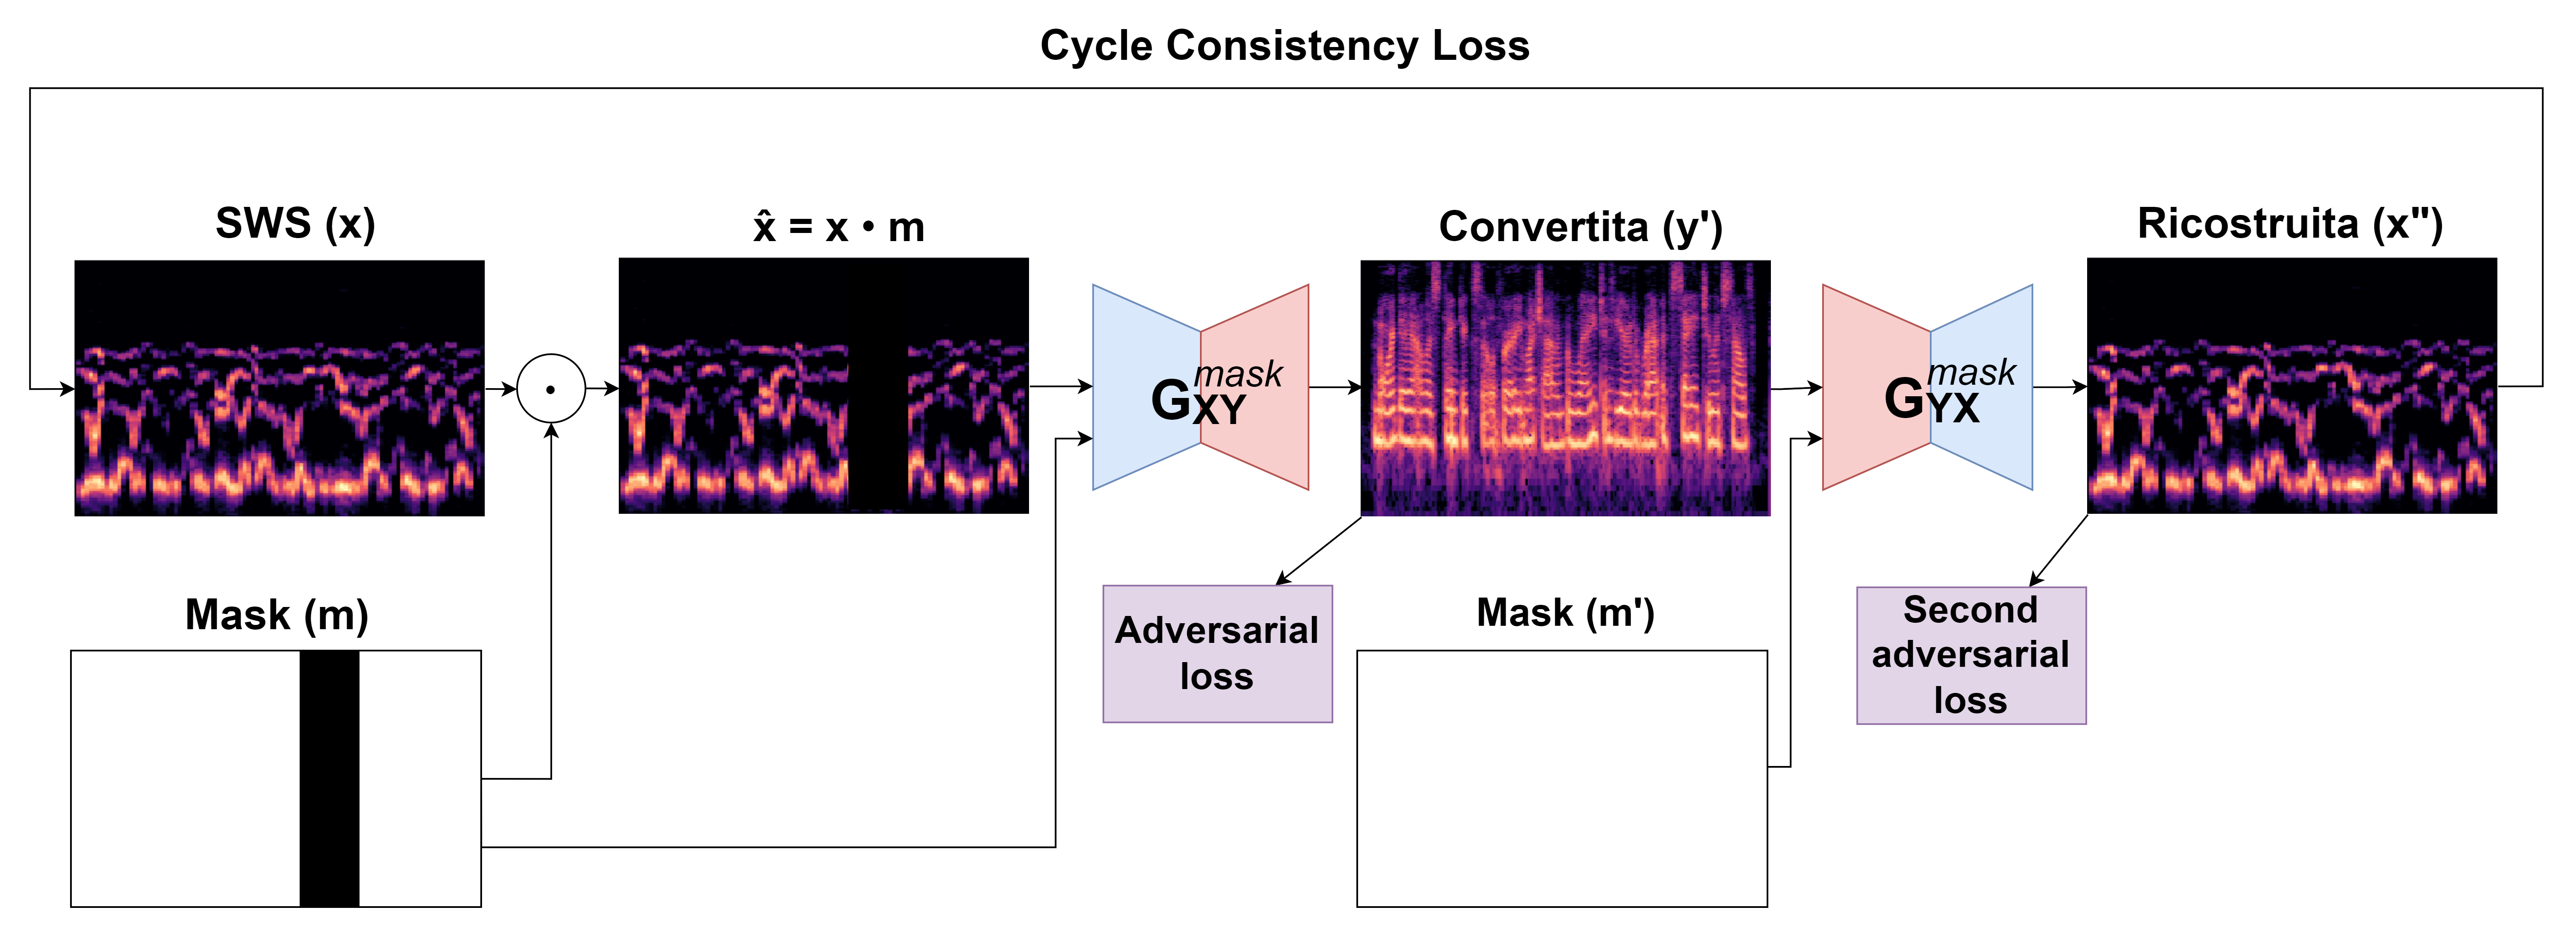
\includegraphics[width=1\linewidth]{figures/MaskCycleGAN-SWS-VC}
			\caption{Ciclo forward dell'architettura proposta impiegando il modulo di riduzione a SWS. Il modello verrà addestrato a trasformare la forma ridotta della voce di $X$ nella voce di $Y$.}
			\label{fig:maskcyclegan-sws-vc}
		\end{figure}
